\section{详细系统设计}
\label{sec:appendix-system-design}

本附录详细描述第~\ref{sec:system-design} 节介绍的 Agent Lightning v1.0 三个组件：API 网关、Rollout 控制器与定制化训练器。

\subsection{API 网关}

API 网关是 Agent Lightning v1.0 的中心组件，刻意保持轻量：一个有状态服务，存储 rollout、模型与事件，并通过最小 API 暴露它们。图~\ref{fig:api-gateway-schema} 总结这些对象及其关系。

\begin{figure}[t]
	\centering
	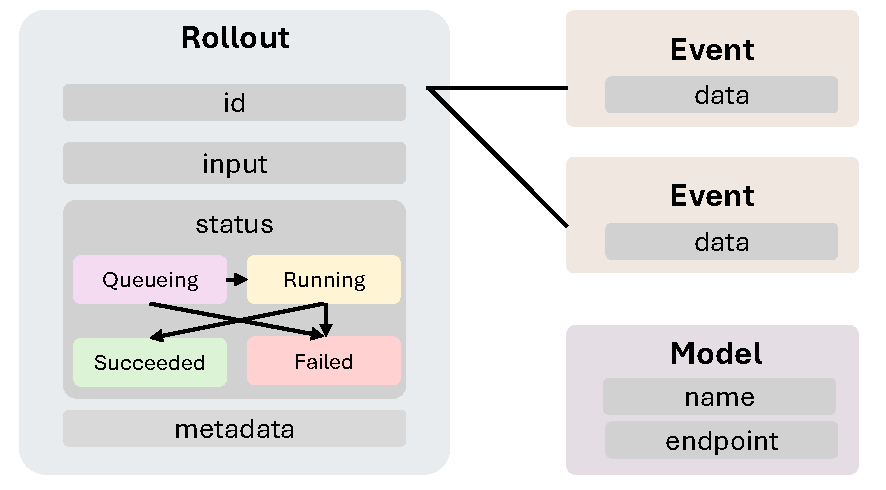
\includegraphics[width=0.5 \linewidth]{figures/agl-lite-schema.pdf}
	\caption{API 网关存储的对象。}
	\label{fig:api-gateway-schema}
\end{figure}

\paragraph{Rollout。}
一次\emph{rollout} 是一次智能体执行，由唯一 rollout ID 标识。它存储输入（源自训练样本）、状态与用户自定义元数据。状态遵循图~\ref{fig:api-gateway-schema} 中的状态机：\texttt{queuing}、\texttt{running} 与终止状态 \texttt{succeeded}、\texttt{failed}。rollout 与训练样本并非一一对应：例如 GRPO~\cite{deepseekmath} 从同一样本生成多次独立 rollout，各自拥有独立 ID 与轨迹。

\paragraph{模型。}
一个\emph{模型}以其名称与地址标识一个 LLM 推理端点。训练器向 API 网关注册模型，网关随后将智能体脚手架请求路由至对应推理服务器。

\paragraph{事件。}
一个\emph{事件}向 rollout 附加任意数据。默认情况下，Agent Lightning v1.0 为每次 LLM 交互记录 \texttt{model\_request} 事件（prompt token ID、响应 token ID 与响应对数概率），并记录智能体通常在 rollout 结束时一次性上报标量奖励的 \texttt{reward} 事件。用户也可以定义自定义事件类型。

\medskip

表~\ref{tab:api-gateway-endpoints} 列出 API 网关的端点，分两类 API：rollout API 与代理 API。

\begin{table}[t]
	\centering
	\small
	\begin{tabular}{@{}lp{0.43\linewidth}p{0.42\linewidth}@{}}
		\toprule
		方法 & 端点 & 说明 \\
		\midrule
		POST & \path|/api/rollouts| & 批量创建 rollout。 \\
		GET & \path|/api/rollouts| & 列出 rollout，可按状态过滤。 \\
		GET & \path|/api/rollouts/{rollout_id}| & 获取单个 rollout。 \\
		PATCH & \path|/api/rollouts/{rollout_id}| & 更新 rollout 状态。 \\
		POST & \path|/api/rollouts/{rollout_id}/attempt/{attempt_id}/events| & 向 rollout 尝试追加事件。 \\
		GET & \path|/api/rollouts/{rollout_id}/events| & 读取 rollout 事件。 \\
		\midrule
		POST & \path|/api/models| & 注册模型端点。 \\
		DELETE & \path|/api/models| & 移除所有已注册模型端点。 \\
		POST & \path|/proxy/rollout/{rollout_id}/attempt/{attempt_id}/mode/{mode}/openai/v1/chat/completions| & 转发 OpenAI 兼容模型调用。 \\
		\bottomrule
	\end{tabular}
	\caption{API 网关端点。}
	\label{tab:api-gateway-endpoints}
\end{table}

\paragraph{Rollout API。}
训练器通过此 API 创建 rollout。Rollout 控制器轮询排队中的 rollout、启动智能体并在执行过程中更新其状态。奖励与其他用户自定义事件以同样方式上传。

\paragraph{代理 API。}
此 API 将来自智能体脚手架的 LLM 调用转发至训练器注册的模型端点。智能体脚手架只需将其 OpenAI 兼容客户端指向代理。由于代理路径嵌入了 rollout ID，每次调用都能自动归属到其 rollout。每次调用的 prompt token ID、响应 token ID 与对数概率被记录为 \texttt{model\_request} 事件，供训练器稍后导出训练。

这一简单 API 将 RL 训练与智能体执行完全解耦：训练器只创建 rollout 与收集轨迹；任何脚手架只需将其 LLM 端点切换到代理即可接入；训练与执行资源可以独立供给，甚至运行在不同地点。

\subsection{Rollout 控制器}

Rollout 控制器在 Kubernetes 之上管理智能体执行。如图~\ref{fig:rollout-controller} 所示，它定期从 API 网关获取活跃 rollout，启动相应智能体任务、监控它们，并通过网关 API 回报状态。其主要后端是 K8s 协调器（K8s Reconciler），面向开源 Kubernetes 集群；为便于调试，还提供面向本地进程池的本地协调器（Local Reconciler）。

\begin{figure}[t]
	\centering
	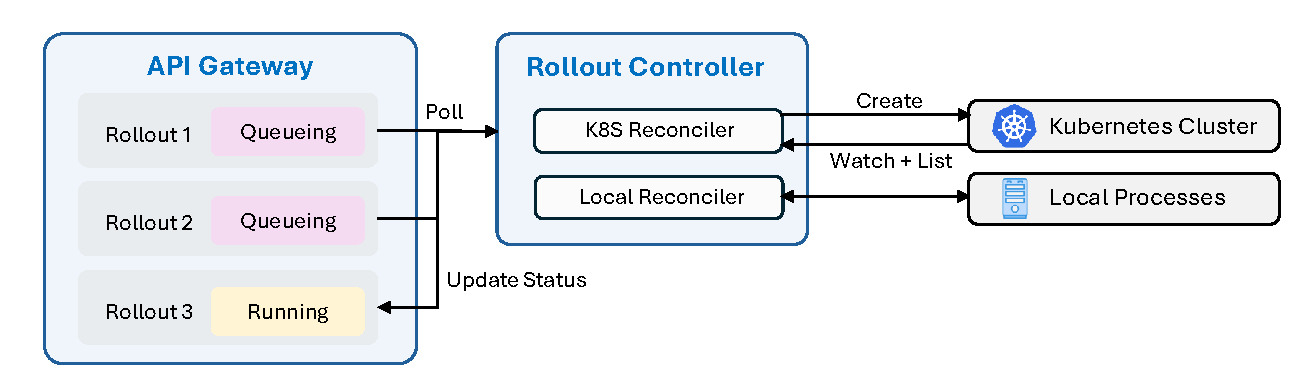
\includegraphics[width=\linewidth]{figures/agl-lite-controller.pdf}
	\caption{Rollout 控制器将 API 网关中的 rollout 状态与以 Kubernetes Job 或本地进程运行的智能体执行进行调和。}
	\label{fig:rollout-controller}
\end{figure}

\paragraph{K8s 协调器。}
对每个尚无对应 Kubernetes Job 的 \texttt{queuing} rollout，它依据用户提供的模板创建一个 Job。它监听 Kubernetes API 的 Job 更新，使终止状态低延迟传播；并周期性列举所有受管 Job 以恢复错过的监听事件——标准 Kubernetes 控制器模式。

\paragraph{本地协调器。}
它在本地进程池中启动智能体。由于直接持有进程句柄，仅周期性轮询即足够，无需单独监听机制。

\paragraph{状态一致性。}
API 网关的 rollout 状态是事实来源。从 Kubernetes 观察到的执行状态可能因网络失败或延迟更新而滞后。K8s 协调器只需在下一周期重试同步，两侧在通信恢复后收敛。这一设计只保证尽力而为的最终一致性。

\subsection{定制化训练器}

定制化训练器基于 VERL~\cite{hybridflow} 构建，在保持轻量设计的同时将训练后端接入 API 网关：每步为当前批次注册 rollout，等待其到达终止状态，然后取回其 \texttt{model\_request} 与 \texttt{reward} 事件并组装为训练样本。它由以下两个组件组成。

\paragraph{专用样本适配器。}
该适配器体现我们对第~\ref{sec:challenges} 节所述挑战的设计选择。
\begin{itemize}
	\item \textbf{样本合并。}我们让 API 网关尽可能简单：不维护服务端请求缓冲区，使训练与部署保持一致。适配器仅在后一次 prompt 是前一次请求与响应的精确 token 级前缀匹配时，才将两次相邻模型请求合并为一个训练样本。
	\item \textbf{优势计算。}适配器在 rollout 层面计算基线与优势，我们认为这是更合理的选择。
	\item \textbf{损失归一化。}适配器实现第~\ref{sec:challenges} 节讨论的 rollout 级 token 均值损失，使每次 rollout 无论样本数多少都携带相等权重。
\end{itemize}

\paragraph{轨迹监控。}
由于智能体训练可能产生奖励黑客、失控轨迹或静默失败，训练器暴露每次训练与验证 rollout 的输入、状态、模型请求、奖励、token/回合统计与自定义事件，执行日志保存在 Kubernetes 中，便于人工或借助 AI 智能体检查，诊断异常行为。
